%!TEX root = main.tex

\newpage
\appendix
\begin{landscape}

\global\pdfpageattr\expandafter{\the\pdfpageattr/Rotate 90}

\section{Appendix A - Gantt diagrams} \label{App:A}

\begin{figure}[!ht]  
\begin{center}  
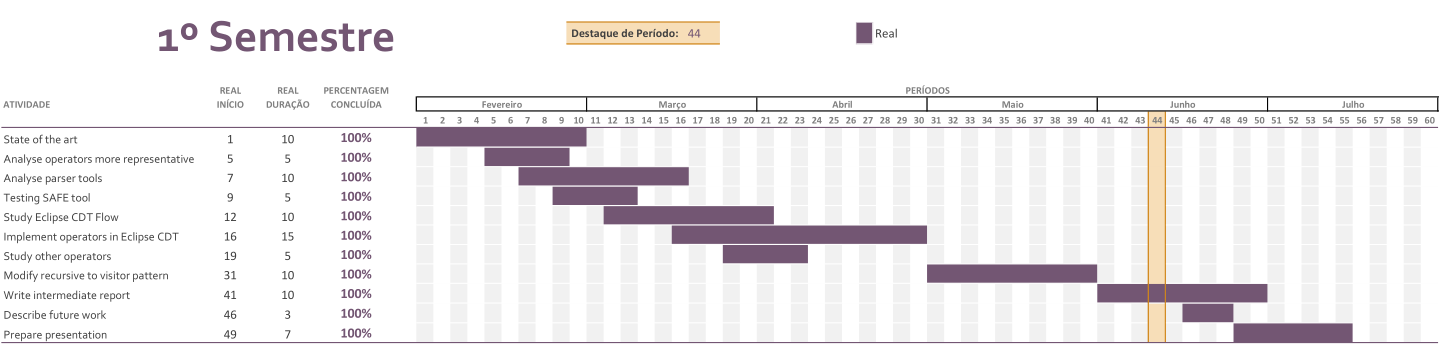
\includegraphics[width=1.6\textwidth]{img/gantt1.png}  
\caption{\small \sl First semester gantt.\label{fig:gantt1}}  
\end{center}  
\end{figure}

\begin{figure}[!ht]  
\begin{center}  
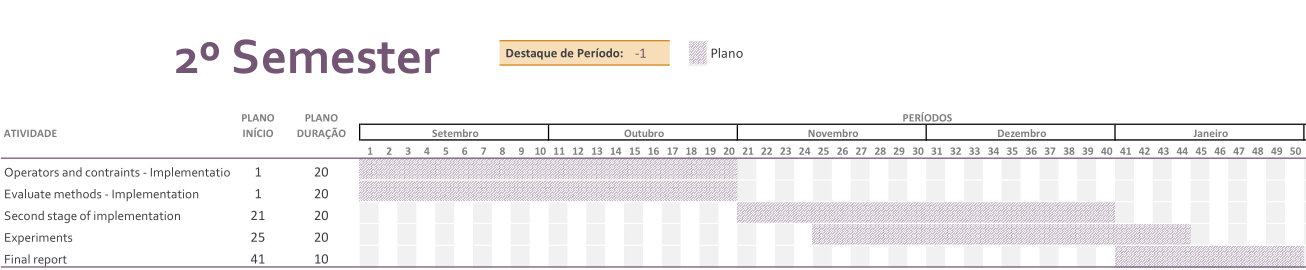
\includegraphics[width=1.6\textwidth]{img/gantt2.png}  
\caption{\small \sl Second semester gantt.\label{fig:gantt2}}  
\end{center}  
\end{figure}

\clearpage

\section{Appendix B - Risks table} \label{App:B}
\begin{figure}[!ht]  
\begin{center}  
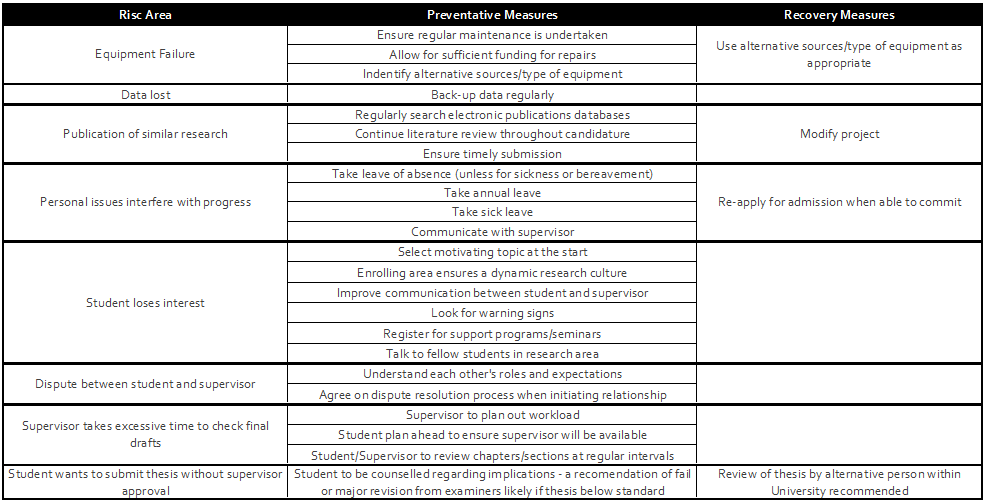
\includegraphics[width=1.5\textwidth]{img/risks.png}  
\caption{\small \sl Risks.\label{fig:risks}}  
\end{center}  
\end{figure}

\end{landscape}
\global\pdfpageattr\expandafter{\the\pdfpageattr/Rotate 0}

\clearpage

\section{Appendix C - Decision Tree} \label{App:C}
\begin{figure}[!ht]  
\begin{center}  
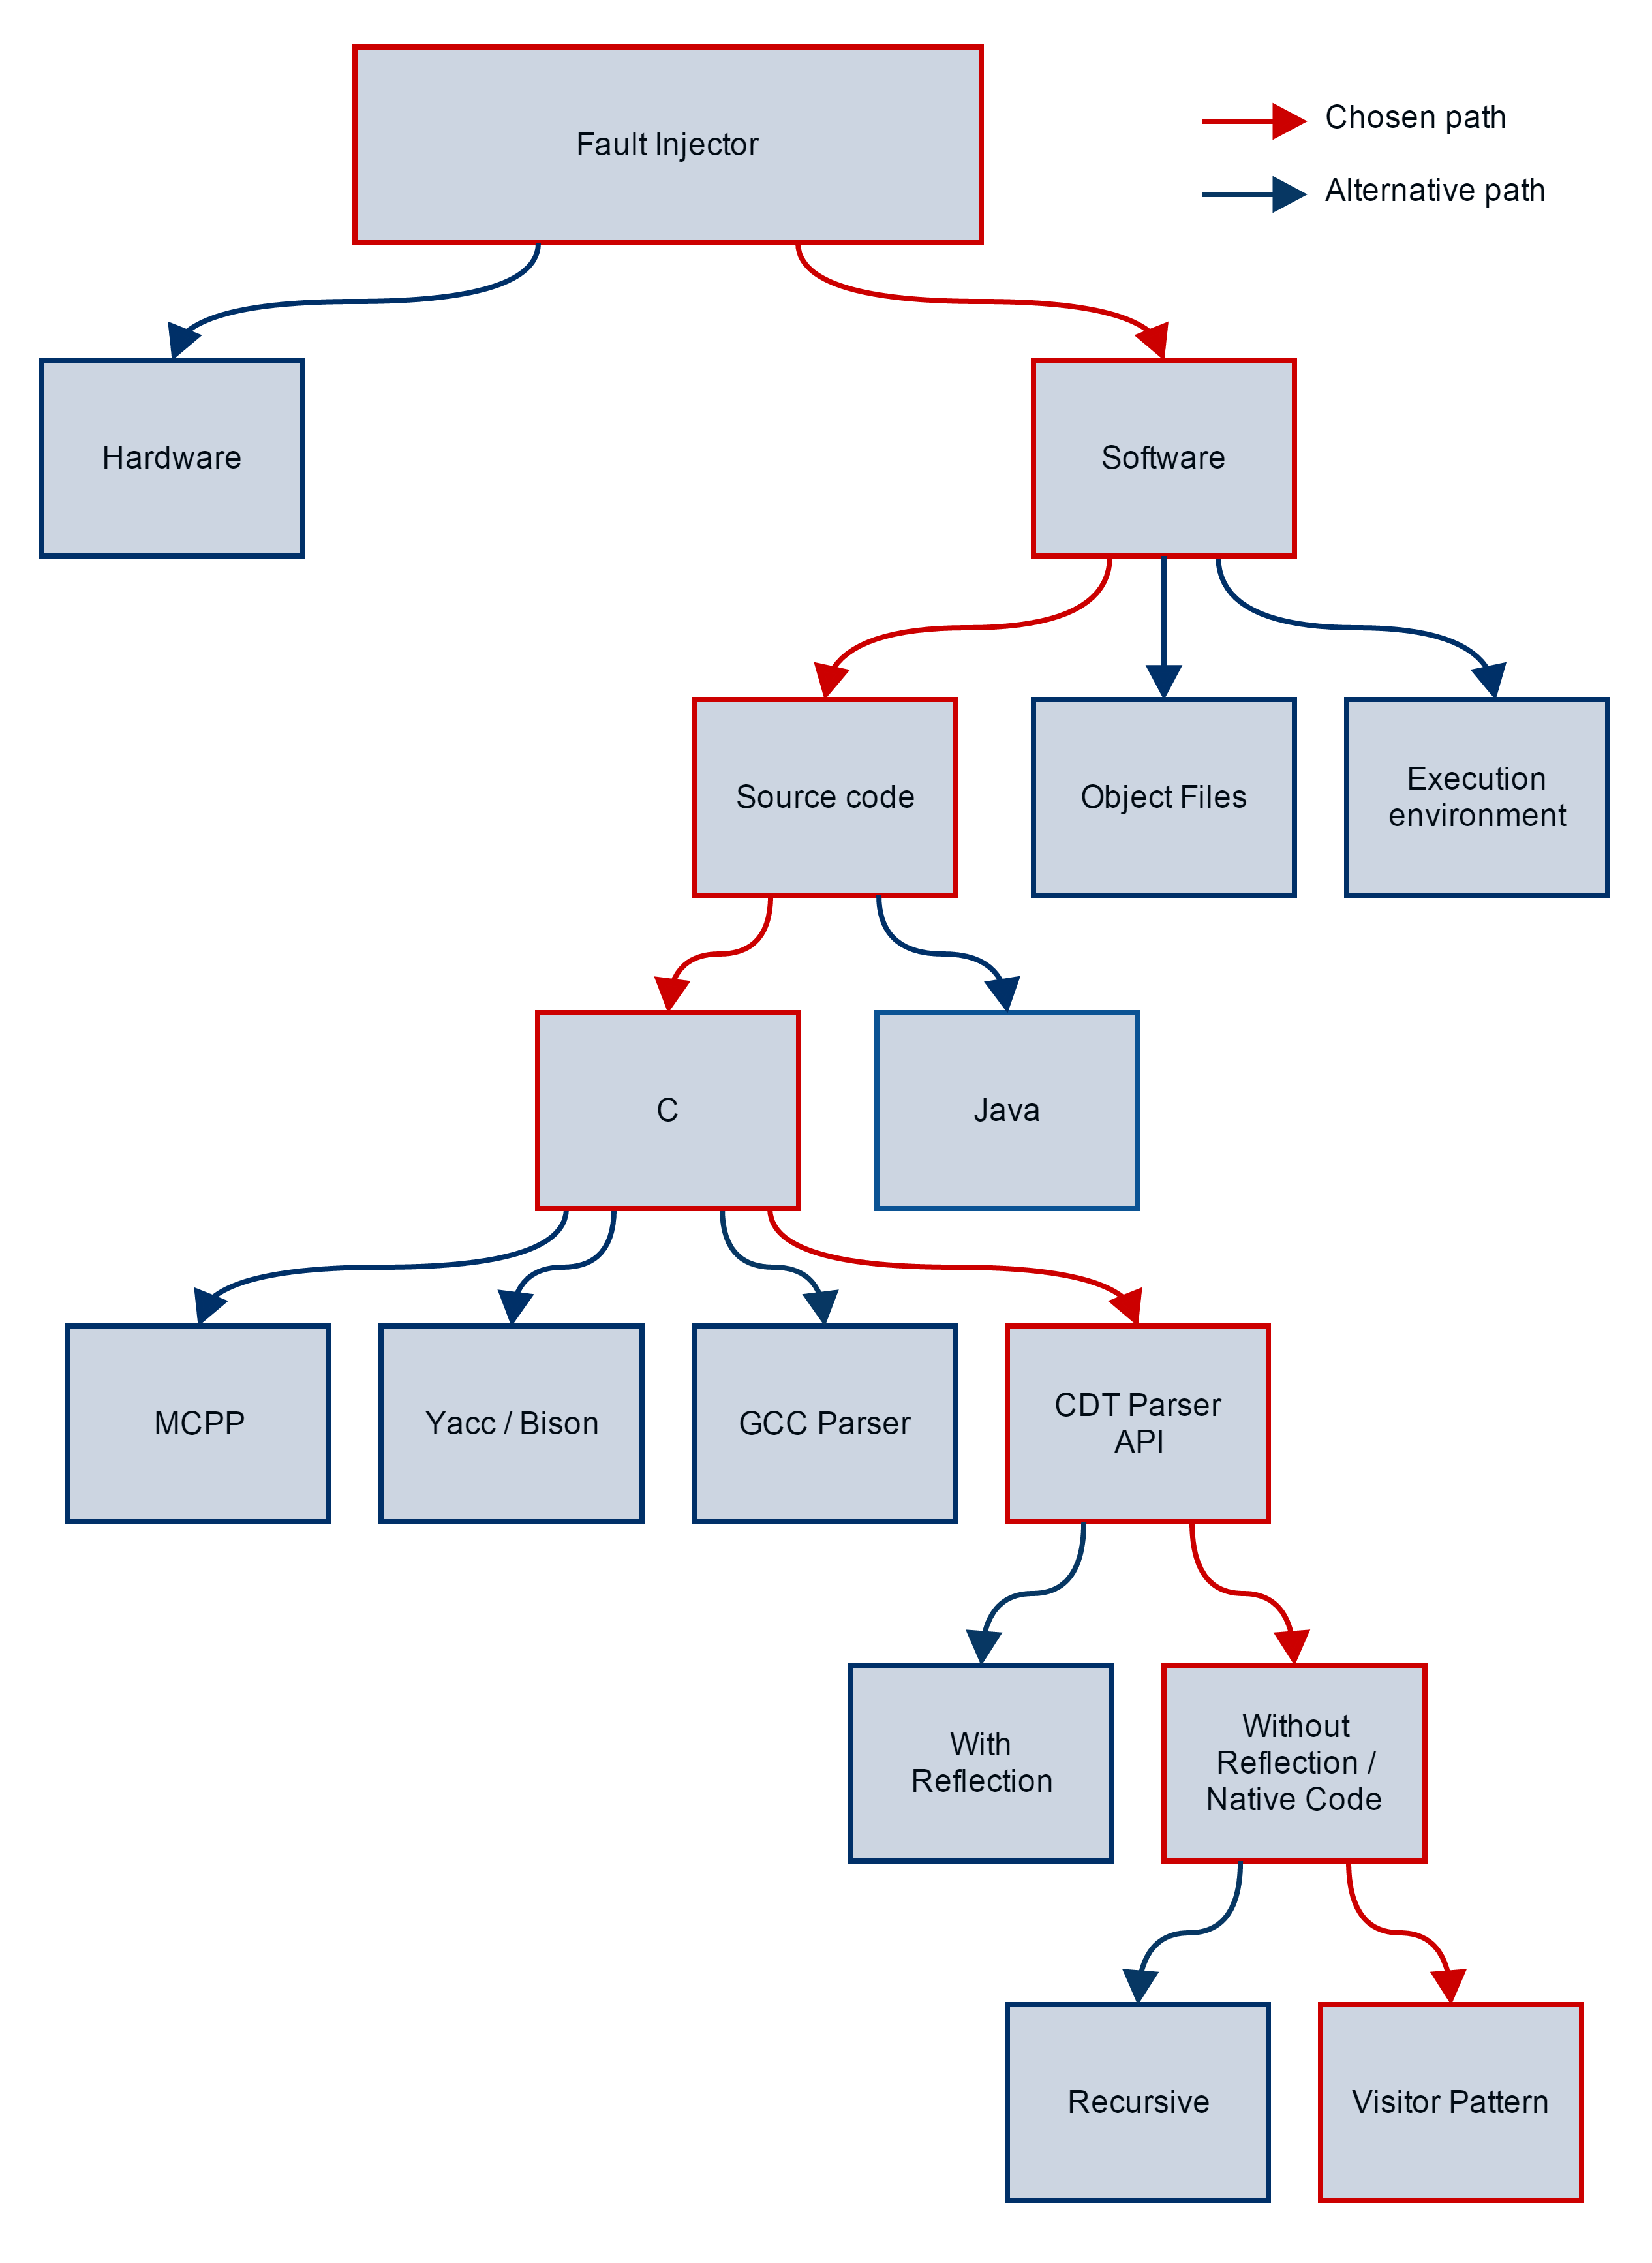
\includegraphics[width=1.1\textwidth]{img/decisions.png}  
\caption{\small \sl Decision Tree.\label{fig:decisions}}  
\end{center}  
\end{figure}

\newpage
